% DOCUMENTO PRINCIPAL

% Este es el fichero principal de este repositorio. No se recomienda editarlo.
% Modifica las plantillas incluidas en los directorios:
% - secciones
% - tablas
% - algoritmos

\documentclass[final,a4paper,11pt,twoside]{class_diss}

\usepackage[full]{textcomp}
\usepackage{graphicx}
\usepackage{amsmath}
\usepackage{amsxtra}
\usepackage{amssymb}
\usepackage{amsthm}
\usepackage{latexsym}
\usepackage{setspace}
\usepackage[margin=3cm]{geometry}
\usepackage[titles]{tocloft}
\usepackage{latexsym}
\usepackage{fancyhdr}
\usepackage{emptypage}
\usepackage[svgnames,dvipsnames,usenames,table,xcdraw]{xcolor}
\usepackage{tikz}
\usepackage[toc,acronym,nonumberlist,xindy={language=spanish-traditional},sanitize=none]{glossaries}
\usepackage[scaled]{helvet}
\usepackage[utf8]{inputenc}
\usepackage[T1]{fontenc}
\usepackage[spanish,es-tabla]{babel}
\usepackage[explicit]{titlesec}
\usepackage{newtxtext}
\usepackage{newtxmath}
\usepackage{stmaryrd}
\usepackage{bbold}
\usepackage[ruled,vlined]{algorithm2e}
\usepackage{algorithmic}
\usepackage{float}
\usepackage{url}
\usepackage{xspace}
\usepackage{booktabs}
\usepackage{multirow}
\usepackage{enumitem}
\usepackage{rotating}
\usepackage{pdflscape}
\usepackage{listings}
\usepackage{placeins}
\usepackage{flafter}
\usepackage{ dsfont }

\theoremstyle{definition}
\newtheorem{definition}{Teorema}[section]
\newcommand{\G}{\mathcal{G}}     % Grafo
\theoremstyle{remark}
\newtheorem*{remark}{Remark}
\DeclareMathOperator*{\argmax}{arg\,max}
\DeclareMathOperator*{\argmin}{arg\,min}
\definecolor{VIU}{RGB}{240, 90, 15}
\definecolor{DESTACADO}{RGB}{130, 34, 145}
\definecolor{CITA}{RGB}{0, 123, 194}

\renewcommand{\algorithmcfname}{Algoritmo}
\renewcommand{\acronymname}{Lista de Acr\'onimos}
\addto\captionsspanish{
    \renewcommand*{\acronymname}{Lista de Acr\'onimos}
}
\newcommand{\inhib}{\relbar\mapsfromchar}
\newcommand{\destacado}[1]{\color{DESTACADO}\textbf{#1}\color{black}\xspace}

\usetikzlibrary{shapes}
\newcommand*\circled[1]{\tikz[baseline=(char.base)]{
    \node[shape=diamond,fill=black!90,inner sep=1pt,minimum size=1cm] (char) {\textcolor{white}{\small\textbf{#1}}};}
}

\pagestyle{fancy}
\fancyhf{}
\fancyhead[LO]{}
\fancyhead[RE]{}
\fancyfoot[C]{}
\renewcommand{\headrulewidth}{0pt}

\fancypagestyle{plain}{
  \fancyhf{}
  \fancyfoot[C]{\circled{\thepage}}
  \renewcommand{\headrulewidth}{0pt}
}

\colorlet{chapnumcolor}{VIU}

\newcommand*{\chapnumfont}{%
  \usefont{T1}{jkp}{b}{n}%
  \fontsize{70}{90}%
  \selectfont%
}

\newcommand*{\chaptitlefont}{%
  \usefont{T1}{qhv}{b}{n}%
  \fontsize{22}{26}%
  \selectfont%
}

\titleformat{name=\chapter}
{\normalfont\huge\bfseries}
{\rlap{\parbox{\textwidth}{\filleft\chapnumfont\color{chapnumcolor}\thechapter}}}
{0pt}
{\rlap{\parbox{0.7\textwidth}{\filright\chaptitlefont #1}}}

\makeglossaries
% GLOSARIO

% Si quieres incluir un glosario y una lista de abreviaturas en tu Trabajo Fin de Máster,
% sigue las instrucciones indicadas en la siguiente URL:
% https://www.overleaf.com/learn/latex/glossaries



\bibliographystyle{apa}

\usepackage[authoryear,sort&compress]{natbib}
\usepackage{hypernat}
\setcitestyle{authoryear}

\usepackage[pdftex,plainpages=false,pdfpagelabels]{hyperref}

\hypersetup{
    linktocpage=true,
    colorlinks=true,
    bookmarks=true,
    citecolor=CITA,
    urlcolor=CITA,
    linkcolor=CITA,
    citebordercolor={1 0 0},
    urlbordercolor={1 0 0},
    linkbordercolor={.7 .8 .8},
    breaklinks=true,
    pdfpagelabels=true,
    }

\setcounter{secnumdepth}{3}
\onehalfspacing
\renewcommand\familydefault{\sfdefault}

\begin{document}

%%%% Incluye la portada oficial%%%%
%% Archivo portada.docx
\cleardoublepage

% Escribe aquí tu frase favorita
\null\vspace{\stretch{2}}
{
\hfill \begin{minipage}{8cm}
\textsl{
\begin{flushright}
    Escribe aquí \\ tu frase favorita.
\end{flushright}
}

% E indica aquí su autor
\begin{flushright}
E indica aquí su autor
\end{flushright}

\end{minipage}
}
\vspace{\stretch{1}}


\pagenumbering{gobble}
% AGRADECIMIENTOS

\cleardoublepage

\normalfont{\huge{\bfseries{Agradecimientos}}}
\vspace{15ex}

% Escribe tus agradecimientos a continuación.
% Se recomienda separar cada párrafo con un \medskip.

Me gustaría agradecer...
\medskip

También quiero destacar...
\medskip

Por último...

\cleardoublepage

\newpage
\pagenumbering{roman}
\setcounter{page}{1}

\pagestyle{fancy}
\fancyhf{}
\fancyhead[LO]{\leftmark}
\fancyhead[RE]{\rightmark}
\fancyfoot[C]{\circled{\thepage}}
\renewcommand{\headrulewidth}{0.4pt}

\pdfbookmark[0]{\contentsname}{contents}

\renewcommand{\cftchapleader}{\cftdotfill{\cftdotsep}}
\renewcommand{\cftchapfont}{\mdseries}
\renewcommand{\cftchappagefont}{\mdseries}

\tableofcontents
\listoffigures
\listoftables

\renewcommand{\listalgorithmcfname}{Índice de algoritmos}
\listofalgorithms
\addcontentsline{toc}{chapter}{Índice de algoritmos}

\newpage
\pagenumbering{arabic}
\setcounter{page}{1}

%\cleardoublepage

\chapter*{Resumen}
\label{resumen}
\addcontentsline{toc}{chapter}{Resumen}

% Escribe aquí 

% INTRODUCCIÓN

\cleardoublepage

\chapter{Introducción}
\label{introduccion}

En los últimos años, los grandes modelos del lenguaje (LLMs) han experimentado un avance significativo, revolucionando diversos campos relacionados con el procesamiento del lenguaje natural (NLP). Estos modelos, entrenados con grandes cantidades de datos, han demostrado una capacidad impresionante para generar texto coherente y relevante en una variedad de contextos. Sin embargo, uno de los desafíos persistentes en el uso de LLMs es su capacidad para manejar información específica y detallada de manera eficiente y precisa.

Una metodología emergente que aborda este desafío es la generación aumentada por recuperación (retrieval augmented generation, RAG). Los sistemas RAG combinan las capacidades generativas de los LLMs con técnicas de recuperación de información, permitiendo a los modelos acceder a bases de datos externas para mejorar la precisión y relevancia de las respuestas generadas. Este enfoque es particularmente útil ya que enriquece el contexto de los LLMs de manera que son capaces de contextualizar mejor el texto que se desea generar.

En esta tesis, se exploran las metodologías de chunkerización y retrieval en el contexto de la Constitución Española. La chunkerización es un proceso crítico que implica dividir un documento en fragmentos manejables, o chunks, que pueden ser más fácilmente procesados por los modelos de lenguaje. Se ha desarrollado un splitter especializado para chunkerizar los artículos de la Constitución Española de manera precisa y coherente. Este trabajo incluye una comparación detallada de diversas metodologías de chunkerización, evaluadas mediante métricas específicas para determinar la eficacia y eficiencia de cada una.

Además, se explicarán brevemente los conceptos fundamentales relacionados con los LLMs y los sistemas RAG, incluyendo embeddings y almacenes vectoriales (vector stores). Estos conceptos son esenciales para comprender cómo se integran las técnicas de recuperación de información con los modelos generativos, mejorando significativamente su rendimiento en tareas específicas.

En resumen, esta tesis busca proporcionar una visión comprensiva de cómo los sistemas RAG pueden ser aplicados de manera efectiva. Para ello, se compararán diferentes metodologías de chunkerización y se culminará con la creación de un agente con la capacidad de contextualizar las preguntas usando la constitución española.

\subsection{Objetivos}

%% OBJETIVOS

\cleardoublepage

\chapter{Objetivos}
\label{objetivos}

Describe aquí el objetivo general de tu Trabajo Fin de Máster y, a continuación, define los objetivos parciales:
\medskip
\begin{enumerate}[label=\destacado{\arabic*.}]
  \setlength\itemsep{1em}
  \item \textbf{Objetivo parcial 1.}

  \item \textbf{Objetivo parcial 2.}

  \item \textbf{Objetivo parcial 3.}
\end{enumerate}

%% METODOLOGÍA

\cleardoublepage

\chapter{Metodología}
\label{metodologia}

% INTRODUCCIÓN

\cleardoublepage

\chapter{Estrategias de chunkerización para LLMs}
\label{Estrategias de chunkerización}

\section{Introducción}
La chunkerización en el ámbito de los modelos de lenguaje de gran escala (LLM) se refiere al proceso de dividir textos extensos en segmentos más manejables, conocidos como \textit{chunks}. Esta técnica es fundamental para mejorar la gestión y el procesamiento de grandes volúmenes de información en aplicaciones de inteligencia artificial que utilizan modelos de lenguaje para entender y generar texto humano.

\textbf{Necesidad de la Chunkerización:} Los modelos de lenguaje, son inherentemente limitados por la cantidad de texto que pueden procesar en una sola instancia debido a restricciones de memoria y capacidad de cálculo. Al descomponer los textos en chunks más pequeños, se facilita que el modelo maneje datos extensos de manera eficiente, permitiendo una evaluación más rápida y precisa.

\textbf{Objetivos de la Chunkerización:} El principal objetivo de la chunkerización es maximizar la relevancia y la precisión del texto procesado. Al dividir el contenido en partes significativas y manejables, se busca preservar la coherencia semántica sin sobrecargar el modelo. Además, esta estrategia es crucial para la indexación efectiva de contenidos en bases de datos vectoriales, lo que mejora la recuperación y relevancia de los resultados en consultas específicas.

\textbf{Retos de la Chunkerización:} A pesar de sus beneficios, la chunkerización presenta varios desafíos. El más significativo es determinar el tamaño óptimo de cada chunk. Si los chunks son demasiado pequeños, pueden perder contexto necesario para una comprensión completa; si son demasiado grandes, pueden exceder las capacidades de procesamiento del modelo y diluir la relevancia del contenido. Otro reto es la selección de los puntos de corte dentro del texto, que debe hacerse de manera que se preserve la integridad del contenido semántico.

La chunkerización es un proceso esencial que requiere un cuidadoso equilibrio entre tamaño de chunk, preservación del contexto y capacidades del modelo. En las siguientes secciones, exploraremos diferentes estrategias y métodos de chunkerización, evaluando sus ventajas y limitaciones en diversos contextos de aplicación.

\section{Consideraciones sobre la Chunkerización}

Al desarrollar una estrategia de chunkerización eficaz, es crucial considerar varios aspectos que influirán en el rendimiento y la eficacia del modelo de lenguaje. A continuación, se detallan algunas de las consideraciones más importantes:

\subsection{Naturaleza del Contenido}
El tipo de contenido que se está indexando es determinante en la selección de la estrategia de chunkerización. Por ejemplo, documentos largos como artículos o libros pueden requerir un enfoque diferente en comparación con contenidos más breves como tuits o mensajes instantáneos. Esta distinción afecta tanto la elección del modelo para crear los embeddings como la estrategia de chunkerización a aplicar.

\subsection{Modelo y Tamaño Óptimo del Chunk}
Dependiendo del modelo utilizado para crear los embeddings, existirán tamaños de chunk en los que el modelo desempeñará mejor. Por ejemplo, algunos modelos están optimizados para trabajar con frases individuales, mientras que otros pueden manejar mejor segmentos de texto más largos. Identificar el tamaño de chunk que maximiza la calidad de los embeddings es crucial para el éxito de la estrategia de chunkerización.

\subsection{Complejidad y Longitud de las Consultas de Usuario}
Las expectativas sobre la longitud y complejidad de las consultas de los usuarios deben guiar la manera en que se chunkeriza el contenido. Si las consultas suelen ser cortas y específicas, es posible que se prefiera chunkerizar el contenido en segmentos más pequeños para reflejar esta especificidad. En cambio, consultas más largas y complejas podrían beneficiarse de chunks más grandes que proporcionen un contexto más amplio.

\subsection{Uso de los Resultados Recuperados}
El propósito final de los chunks recuperados también juega un papel crucial. Dependiendo de si los resultados serán utilizados para búsqueda semántica, respuesta a preguntas, resumen, o cualquier otro fin, la estrategia de chunkerización podría variar para optimizar la relevancia y utilidad de la información recuperada.

\subsection{Limitaciones Técnicas}
Las limitaciones técnicas, como el número máximo de tokens que el modelo puede procesar en una sola instancia o las restricciones de memoria, son críticas para definir el tamaño de los chunks. Estas limitaciones no solo afectan cómo se chunkeriza el contenido sino también cómo se procesa posteriormente en el modelo.

Estas consideraciones son fundamentales para desarrollar una estrategia de chunkerización que no solo sea eficiente sino también efectiva en términos de mejorar la relevancia y precisión de las respuestas del modelo.

\section{Estrategias de Chunkerización}

La chunkerización puede implementarse de diversas maneras, cada una con sus propios beneficios y desafíos. A continuación, exploramos algunas de las estrategias más comunes y cómo pueden optimizarse según diferentes necesidades y contextos.

\subsection{Chunkerización de Tamaño Fijo}

Esta estrategia consiste en dividir el texto en segmentos de un tamaño predeterminado, medido en número de tokens o carácteres. La principal ventaja de este método es su simplicidad y facilidad de implementación, ya que no requiere un análisis profundo del contenido. Sin embargo, un desafío significativo es que puede cortar frases a la mitad, perdiendo contexto o generando chunks que carecen de sentido por sí solos. Para mitigar esto, se puede optar por incluir una superposición entre los chunks, donde el final de un chunk se superpone con el inicio del siguiente, ayudando a preservar el contexto (overload).

\begin{figure}[h]
\centering
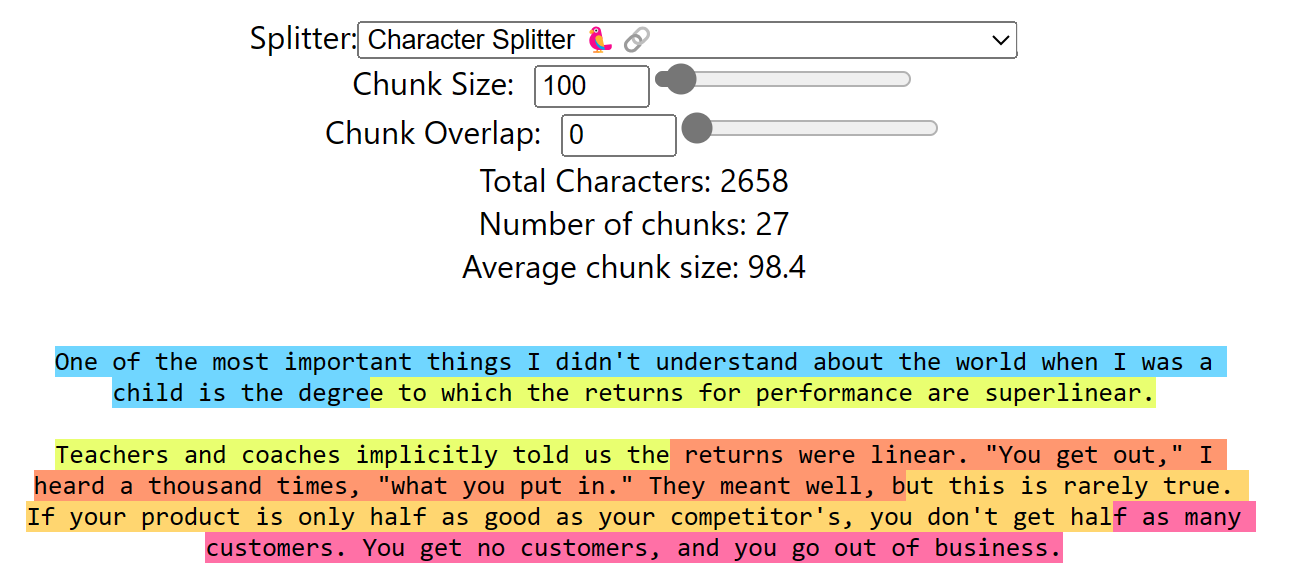
\includegraphics[width=0.8\textwidth]{figuras/capitulo4/character_splitter_100_0.png}
\caption{Ejemplo de chunkerización tamaño fijo sin overload}
\label{fig:imagen_fijo}
\end{figure}

\begin{figure}[h]
\centering
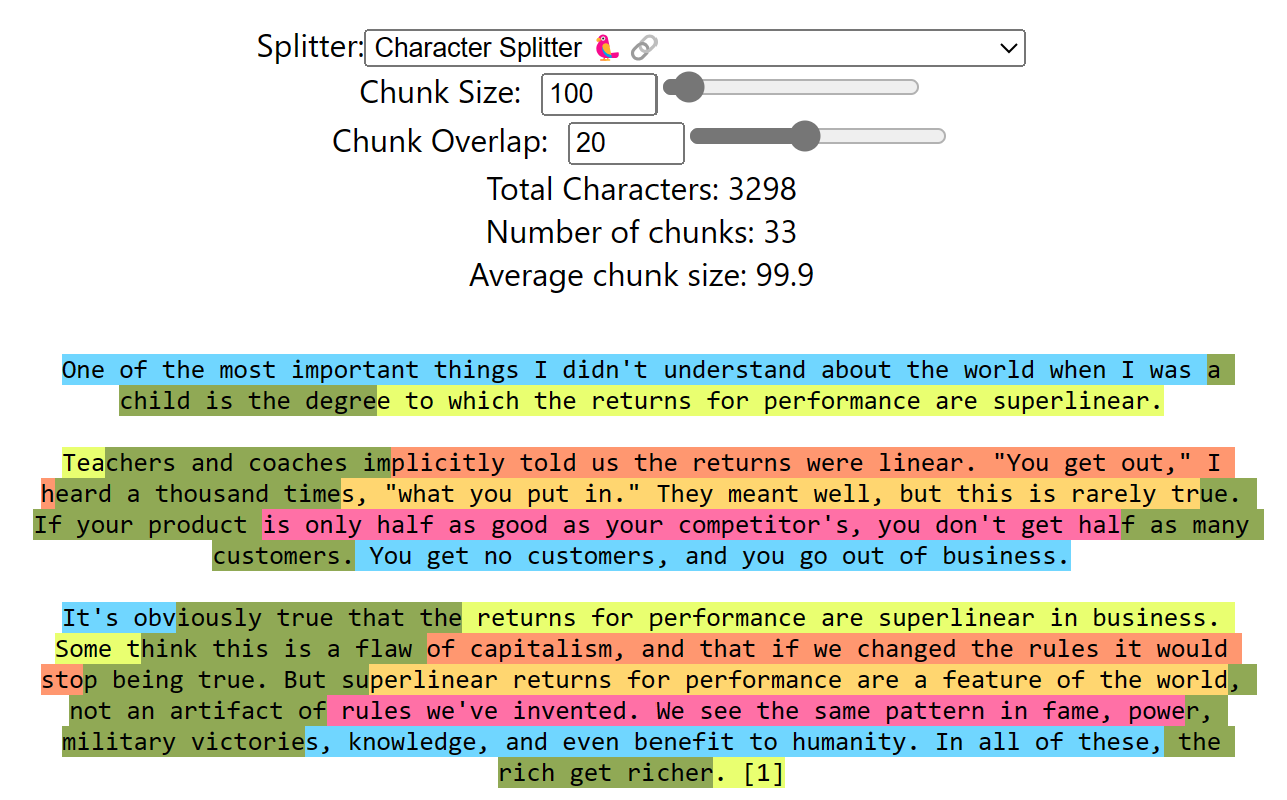
\includegraphics[width=0.8\textwidth]{figuras/capitulo4/character_splitter_100_20.png}
\caption{Ejemplo de chunkerización tamaño fijo con overload}
\label{fig:imagen_fijo_overload}
\end{figure}

\subsection{Chunkerización Consciente del Contenido}

A diferencia de la chunkerización de tamaño fijo, este método tiene en cuenta el contenido textual para determinar los puntos de corte. La chunkerización consciente del contenido puede basarse en la detección de fronteras naturales en el texto, como finales de oraciones o párrafos, asegurando que cada segmento contenga una unidad completa de información. Esto ayuda a mantener la coherencia semántica de los chunks, haciendo que cada uno sea significativo por sí mismo y mejore la calidad de las incrustaciones generadas por el modelo. Este método es particularmente útil en documentos con una estructura clara y bien definida, como artículos académicos o reportes técnicos.

\subsection{Chunkerización Recursiva}

Este enfoque implica un proceso iterativo y jerárquico de dividir el texto en chunks. Inicialmente, el texto se divide utilizando un criterio de separación amplio, y si los chunks resultantes aún son demasiado grandes o no cumplen con ciertos criterios, el proceso se repite en cada chunk hasta alcanzar el tamaño o la estructura deseada. La chunkerización recursiva es útil en textos largos y complejos donde los niveles múltiples de división permiten manejar mejor la diversidad y complejidad del contenido.

\begin{figure}[!h]
\centering
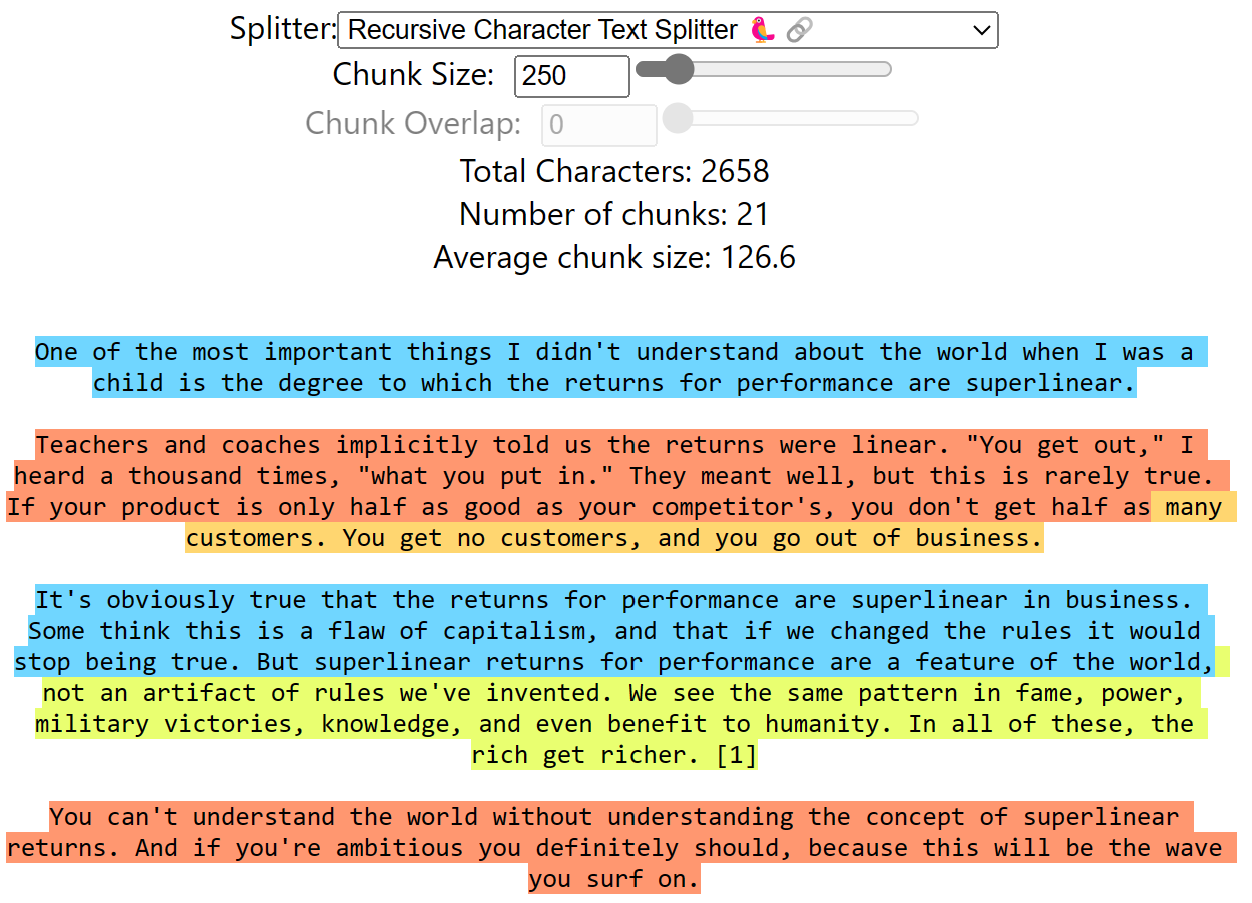
\includegraphics[width=0.8\textwidth]{figuras/capitulo4/recursive_character_splitter_250_0.png}
\caption{Ejemplo de chunkerización recursiva}
\label{fig:imagen_recursiva}
\end{figure}

\subsection{Chunkerización Especializada}

Esta estrategia se adapta a formatos de contenido específicos que requieren un tratamiento particular, como puede ser el caso de textos en Markdown o LaTeX. La chunkerización especializada reconoce y respeta la estructura y sintaxis propias de estos formatos, asegurando que los chunks resultantes conserven la integridad y funcionalidad del texto original. Por ejemplo, en un documento LaTeX, los chunks podrían definirse para encapsular secciones completas o subsecciones, preservando las etiquetas y comandos propios del formato.

Cada una de estas estrategias tiene sus propias fortalezas y puede ser más adecuada para diferentes tipos de textos y aplicaciones. La elección de una estrategia de chunkerización debe basarse en una evaluación cuidadosa de los requisitos del proyecto, la naturaleza del contenido y los objetivos específicos del sistema de procesamiento de lenguaje natural.

\begin{figure}[!h]
\centering
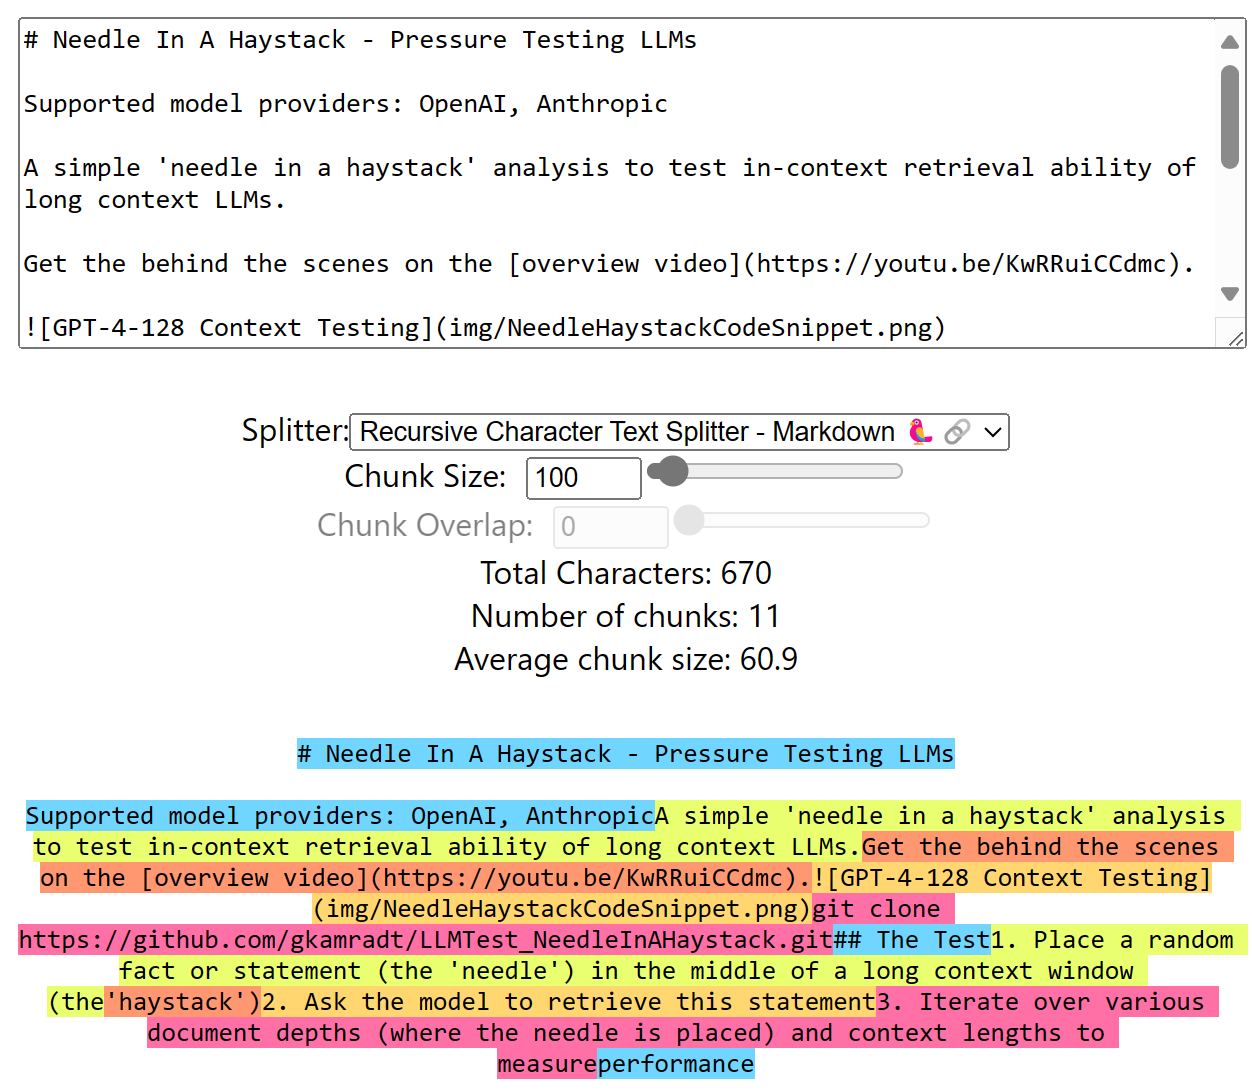
\includegraphics[width=0.8\textwidth]{figuras/capitulo4/character_md_100.png}
\caption{Ejemplo de chunkerización Especializada}
\label{fig:imagen_chunk_md}
\end{figure}

\subsection{Chunkerización Semántica}

La chunkerización semántica es una técnica avanzada que divide el texto en unidades basadas en la relevancia semántica, utilizando modelos de creación de embeddings para evaluar la similitud entre segmentos de texto.

\subsubsection{Implementación y Ventajas}
Esta estrategia se implementa mediante la transformación de texto en representaciones vectoriales y el cálculo de su similitud, agrupando segmentos similares. Es especialmente útil para mantener la coherencia del contenido en tareas de recuperación de información y análisis de texto.

\subsubsection{Desafíos y Aplicaciones}
A pesar de su efectividad, enfrenta desafíos como la alta demanda computacional y la dificultad en determinar umbrales de similitud óptimos. Su aplicación es ideal en sistemas de búsqueda semántica y en el análisis de textos complejos en contextos académicos o de investigación.


\section{Conclusiones}
La chunkerización es fundamental para mejorar la eficiencia y precisión en aplicaciones relacionadas con LLM. No existe una solución única para todos los casos, por lo que es crucial evaluar cada situación individualmente para encontrar la estrategia más efectiva.

%% RESULTADOS Y DISCUSION 

\cleardoublepage

\chapter{Resultados y Discusión}
\label{resultados-y-discusion}

%% CONCLUSIONES

\chapter{Conclusiones}
\label{conclusiones}

\begin{enumerate}[label=\destacado{\arabic*.}]
  \setlength\itemsep{1em}
  \item Conclusión 1.

  \item Conclusión 2.

  \item Conclusión 3.
\end{enumerate}

%% LIMITACIONES Y PERSPECTIVAS DE FUTURO

\cleardoublepage

\chapter{Limitaciones y\\ Perspectivas de Futuro}
\label{limitaciones-y-futuro}


\cleardoublepage
\phantomsection

\printglossary[type=\acronymtype]
\printglossary

\appendix
% APÉNDIZES

% Escribe cada apéndize como si fuera un capítulo más.

\chapter{Apéndize A}
\label{apendize-a}

Figura relativa al benchmark de LLMs.

\begin{figure}[!h]
\centering
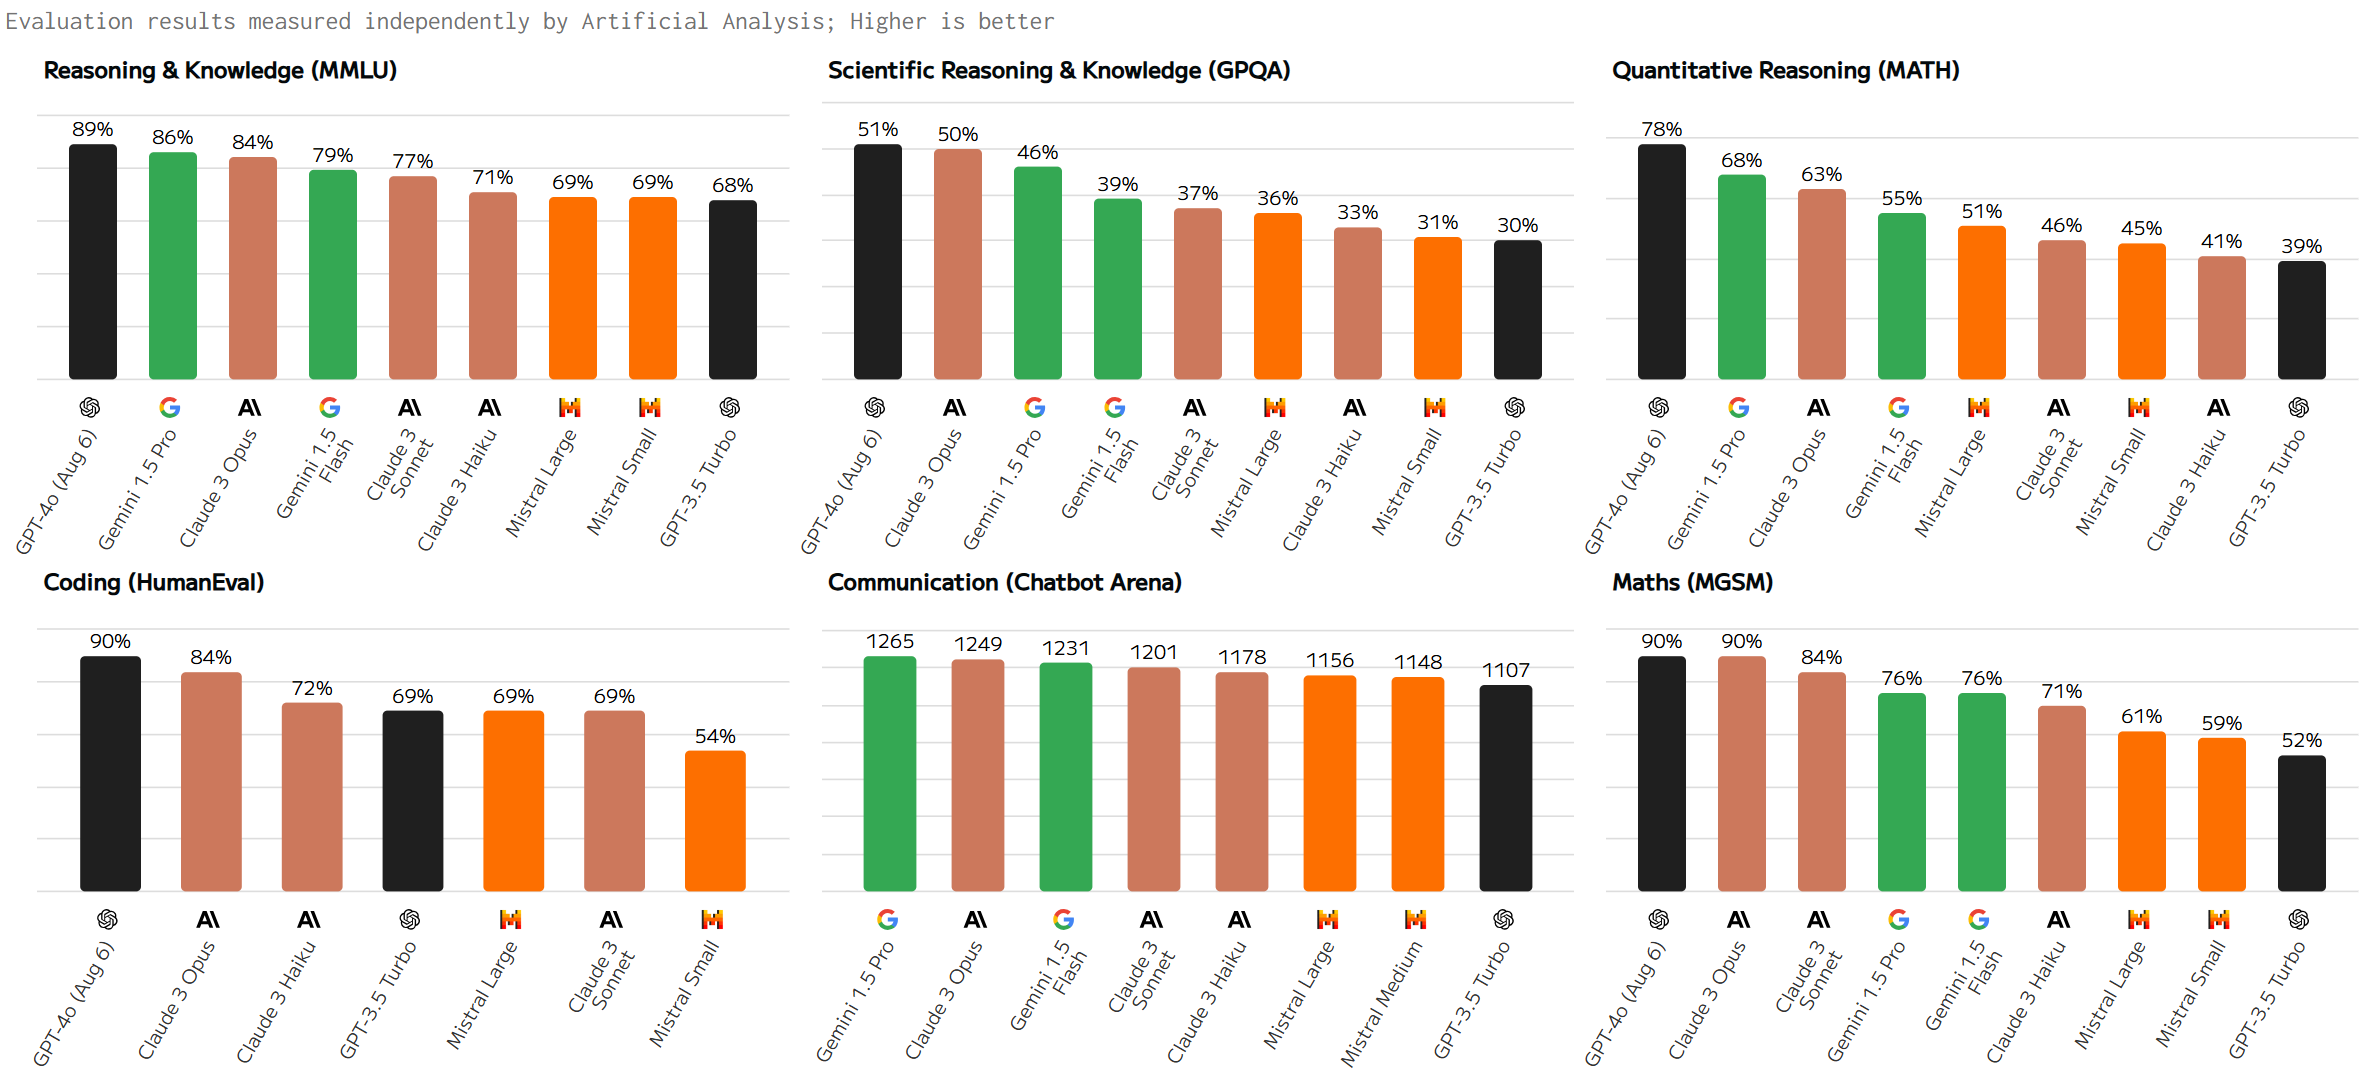
\includegraphics[width=1.1\textwidth,angle=90]{figuras/capitulo6/benchmark.png}
\caption{Benchmark sobre distintas métricas para evaluar LLMs. \citep{artificialanalysis}}
\label{fig:benchmark}
\end{figure}


\begin{singlespace}
\begin{footnotesize}
\begin{twocolumn}
\bibdata{bibliografia}
\bibliography{bibliografia}
\addcontentsline{toc}{chapter}{Bibliografía}
\end{twocolumn}
\end{footnotesize}
\end{singlespace}

\end{document}
